\documentclass{beamer}
\usepackage[utf8]{inputenc}
\usepackage{amsmath}

\title{Problema de Transporte: Balanceo del modelo de transporte}
\author{Ricardo Largaespada}
\date{\today}

\begin{document}

\frame{\titlepage}

\begin{frame}{Balanceo del Modelo de Transporte}
    La representación de la tabla de transporte asume que el modelo está balanceado, es decir, que la demanda total es igual a la oferta total.
    \begin{itemize}
        \item Si el modelo está desbalanceado, se puede agregar un origen o un destino ficticio para restaurar el balance.
    \end{itemize}
\end{frame}

\begin{frame}{Ejemplo 5.1-2: Modelo de MG}
    \begin{itemize}
        \item Suponga que la capacidad de la planta de Detroit es de 1300 automóviles (en lugar de 1500).
        \item La oferta total es de 3500 automóviles, menor que la demanda total de 3700.
        \item Esto significa que no se podrá satisfacer toda la demanda en Denver y Miami.
        \item Para balancear el modelo, se agrega un origen ficticio con una capacidad de 200 automóviles ($3700 - 3500$).
        \item El costo de transporte por unidad desde la planta ficticia a los destinos es cero, ya que la planta no existe.
    \end{itemize}
\end{frame}

\begin{frame}{Representación Gráfica del Ejemplo}
    \begin{center}
        \includegraphics[width=0.8\textwidth]{ruta_de_transporte.png} % Reemplaza con la ruta de la imagen generada o insertada
    \end{center}
    \textbf{Figura 5.2}: Solución óptima del modelo de transporte de MG Auto.
\end{frame}

\begin{frame}{Interpretación de los Resultados}
    \begin{itemize}
        \item \textbf{Oferta total}: 3500 automóviles.
        \item \textbf{Demanda total}: 3700 automóviles.
        \item \textbf{Planta ficticia}: Se agrega para satisfacer la demanda excedente de 200 automóviles.
        \item \textbf{Destinos}: Se observa cómo se distribuye el transporte hacia Denver y Miami para cumplir con las necesidades.
    \end{itemize}
\end{frame}

\begin{frame}{Tabla 5.4: Modelo de MG con una Planta Ficticia}
\begin{center}
    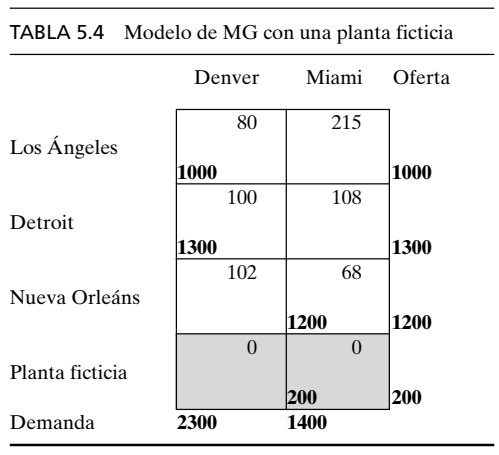
\includegraphics[scale=1]{images/transporte01.png}
\end{center}
    \vspace{0.3cm}
    \textbf{Descripción:} La solución muestra que la planta ficticia envía 200 automóviles a Miami para satisfacer su demanda.
\end{frame}

\begin{frame}{Explicación del Balanceo con Planta Ficticia}
    \begin{itemize}
        \item La planta ficticia permite cubrir la demanda adicional de 200 automóviles en Miami.
        \item El costo de transporte desde esta planta ficticia es cero, ya que no existe en realidad.
        \item Este método ayuda a balancear el modelo cuando la oferta es menor que la demanda total.
    \end{itemize}
\end{frame}

\begin{frame}{Tabla 5.5: Modelo de MG con un Destino Ficticio}
\begin{center}
    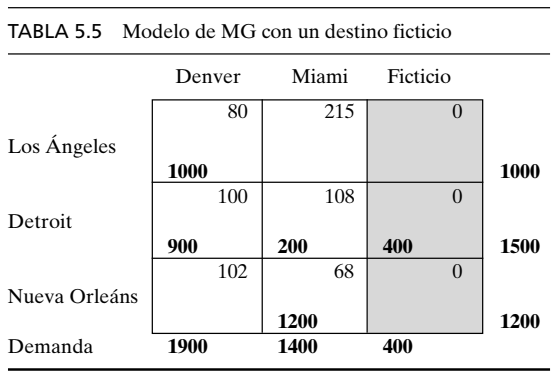
\includegraphics[scale=1]{images/transporte02.png}
\end{center}
    \vspace{0.3cm}
    \textbf{Descripción:} En este modelo, se agrega un destino ficticio con una penalización alta para indicar que hay demanda insatisfecha.
\end{frame}

\begin{frame}{Explicación del Balanceo con Destino Ficticio}
    \begin{itemize}
        \item Este modelo permite identificar claramente la cantidad de demanda que no puede ser satisfecha.
        \item Se usa una penalización de costo alto para señalar la escasez en destinos reales, asegurando que la demanda excedente sea reconocida en el modelo.
        \item Este método es útil cuando no se puede balancear con una planta ficticia o cuando la demanda supera la oferta.
    \end{itemize}
\end{frame}

\end{document}